\chapter{Risultati e discussione}
\label{ch:risultati}

Nelle tabelle di questo capitolo le metriche sono riportate come valori compresi tra $0$ e $1$; le differenze discusse nel testo sono espresse in punti percentuali (ad esempio, una differenza di $0.05$ corrisponde a $5$ punti). Oltre alle metriche descritte nella Sezione~\ref{sec:metriche-valutazione}, le tabelle riportano la Precision macro sulle classi note.

\section{Risultati sul dataset Oxford-IIIT Pet}
\label{sec:pet}

\subsection*{Analisi Macro-drop}

Come mostrato in Figura~\ref{fig:macro-dropout-pet}, il macro-drop non produce un trend di degradazione 
riconoscibile: per tutte le architetture le curve oscillano entro una banda ristretta al variare della percentuale 
di rimozione, senza una direzione definita.

\begin{figure}[!ht]
    \centering
    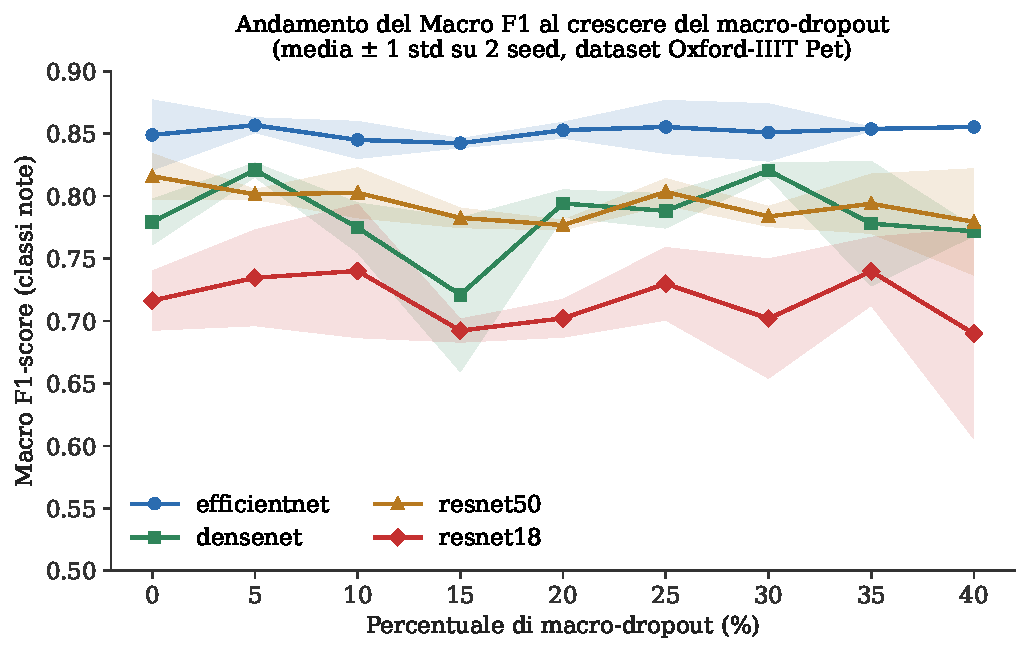
\includegraphics[width=0.75\textwidth]{figures/macro_dropout_f1.pdf}
    \caption{Andamento del Macro F1-score al variare della percentuale di macro-drop, per le quattro architetture testate sul dataset Oxford-IIIT Pet (in tale scenario tutte le classi del dataset rimangono rappresentate nel training set). Le bande rappresentano $\pm 1$ deviazione standard calcolata su due seed (42, 777).}
    \label{fig:macro-dropout-pet}
\end{figure}

\FloatBarrier

\begin{table}[!ht]
    \centering
    \small
    \caption{Accuracy, Precision e F1-score al variare della percentuale di macro-drop, 
    per le quattro architetture sul dataset Oxford-IIIT Pet. Valori riportati come media $\pm$ deviazione standard su due seed (42, 777).}
    \label{tab:metriche-pet-macro}
    \begin{tabular}{llccc}
        \toprule
        \textbf{Modello} & \textbf{Drop \%} & \textbf{Accuracy} & \textbf{Precision} & \textbf{F1-score} \\
        \midrule
        \multirow{3}{*}{EfficientNet} & 0  & $0.851 \pm 0.029$ & $0.862 \pm 0.021$ & $0.849 \pm 0.028$ \\
                                       & 20 & $0.853 \pm 0.009$ & $0.868 \pm 0.001$ & $0.853 \pm 0.006$ \\
                                       & 40 & $0.855 \pm 0.002$ & $0.864 \pm 0.000$ & $0.855 \pm 0.001$ \\
        \midrule
        \multirow{3}{*}{DenseNet}     & 0  & $0.780 \pm 0.017$ & $0.806 \pm 0.010$ & $0.779 \pm 0.018$ \\
                                       & 20 & $0.797 \pm 0.011$ & $0.820 \pm 0.007$ & $0.794 \pm 0.011$ \\
                                       & 40 & $0.772 \pm 0.004$ & $0.799 \pm 0.004$ & $0.772 \pm 0.003$ \\
        \midrule
        \multirow{3}{*}{ResNet50}     & 0  & $0.818 \pm 0.017$ & $0.836 \pm 0.009$ & $0.816 \pm 0.018$ \\
                                       & 20 & $0.777 \pm 0.006$ & $0.805 \pm 0.002$ & $0.777 \pm 0.004$ \\
                                       & 40 & $0.781 \pm 0.038$ & $0.810 \pm 0.027$ & $0.779 \pm 0.043$ \\
        \midrule
        \multirow{3}{*}{ResNet18}     & 0  & $0.719 \pm 0.022$ & $0.763 \pm 0.011$ & $0.716 \pm 0.024$ \\
                                       & 20 & $0.704 \pm 0.015$ & $0.758 \pm 0.011$ & $0.702 \pm 0.015$ \\
                                       & 40 & $0.683 \pm 0.087$ & $0.745 \pm 0.051$ & $0.690 \pm 0.084$ \\
        \bottomrule
    \end{tabular}
\end{table}

\FloatBarrier

I valori riportati in Tabella~\ref{tab:metriche-pet-macro} confermano quanto osservato graficamente: Accuracy, Precision e F1-score restano stabili tra lo $0\%$ e il $40\%$ di macro-drop per ciascuna architettura, 
con variazioni contenute di pochi punti percentuali. Questo risultato è atteso, poiché la riduzione uniforme degli esempi in ogni classe mantiene invariata la distribuzione relativa del dataset, 
lasciando pressoché inalterato il problema di classificazione anche con un numero minore di esempi di training.

Un'eccezione riguarda ResNet18 al $40\%$ di drop, dove la deviazione standard tra i due seed risulta sensibilmente più elevata rispetto agli altri casi ($\pm 0.087$ in Accuracy), 
segnale di una maggiore sensibilità di questa architettura al rumore di ottimizzazione e all'inizializzazione casuale dei parametri delle head lineari, anche a fronte di una riduzione uniforme dei campioni.
\FloatBarrier

\clearpage

\subsection*{Analisi Micro-drop}

Come mostrato in Figura~\ref{fig:micro-dropout-pet} e in Tabella~\ref{tab:metriche-pet}, il micro-drop produce un trend di degradazione marcato: 
il Macro F1-score\footnote{Media semplice dell'F1-score calcolato per ogni classe, limitatamente alle classi presenti nel training set (escluse quindi le razze completamente rimosse dal micro-drop).} 
diminuisce al crescere della percentuale di rimozione delle classi, con intensità diverse tra le quattro architetture testate sul dataset Oxford-IIIT Pet.

\begin{figure}[htbp]
    \centering
    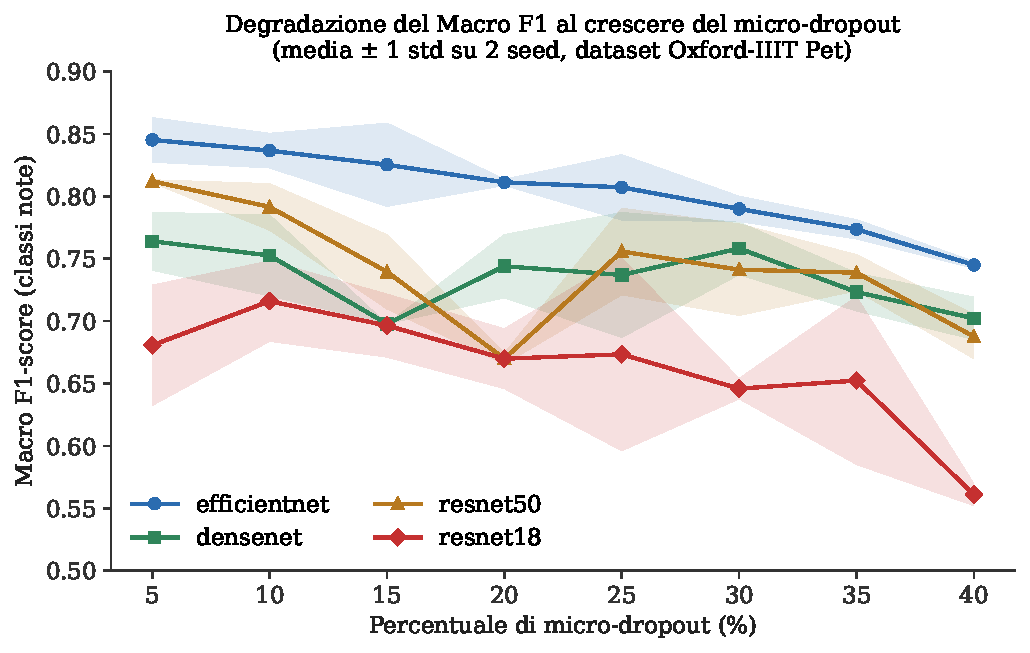
\includegraphics[width=0.85\textwidth]{figures/micro_dropout_f1.pdf}
    \caption{Andamento del Macro F1-score sulle classi note al variare della percentuale di micro-drop, per le quattro architetture testate sul dataset Oxford-IIIT Pet. Le bande rappresentano $\pm 1$ deviazione standard calcolata su due seed (42, 777).}
    \label{fig:micro-dropout-pet}
\end{figure}

\begin{table}[!htb]
    \centering
    \small
    \caption{Accuracy (globale sull'intero test set), Precision (macro, classi note) e F1-score (macro, classi note) al variare della percentuale di micro-drop, per le quattro architetture sul dataset Oxford-IIIT Pet. Valori riportati come media $\pm$ deviazione standard su due seed (42, 777).}
    \label{tab:metriche-pet}
    \begin{tabular}{llccc}
        \toprule
        \textbf{Modello} & \textbf{Drop \%} & \textbf{Accuracy} & \textbf{Precision} & \textbf{F1-score} \\
        \midrule
        \multirow{3}{*}{EfficientNet} & 0  & $0.851 \pm 0.029$ & $0.862 \pm 0.021$ & $0.849 \pm 0.028$ \\
                                       & 20 & $0.753 \pm 0.014$ & $0.798 \pm 0.009$ & $0.811 \pm 0.002$ \\
                                       & 40 & $0.633 \pm 0.016$ & $0.699 \pm 0.005$ & $0.745 \pm 0.003$ \\
        \midrule
        \multirow{3}{*}{DenseNet}     & 0  & $0.780 \pm 0.017$ & $0.806 \pm 0.010$ & $0.779 \pm 0.018$ \\
                                       & 20 & $0.691 \pm 0.015$ & $0.750 \pm 0.007$ & $0.744 \pm 0.025$ \\
                                       & 40 & $0.592 \pm 0.023$ & $0.672 \pm 0.016$ & $0.702 \pm 0.017$ \\
        \midrule
        \multirow{3}{*}{ResNet50}     & 0  & $0.818 \pm 0.017$ & $0.836 \pm 0.009$ & $0.816 \pm 0.018$ \\
                                       & 20 & $0.628 \pm 0.012$ & $0.708 \pm 0.025$ & $0.670 \pm 0.004$ \\
                                       & 40 & $0.578 \pm 0.022$ & $0.684 \pm 0.007$ & $0.688 \pm 0.018$ \\
        \midrule
        \multirow{3}{*}{ResNet18}     & 0  & $0.719 \pm 0.022$ & $0.763 \pm 0.011$ & $0.716 \pm 0.024$ \\
                                       & 20 & $0.628 \pm 0.008$ & $0.673 \pm 0.010$ & $0.670 \pm 0.024$ \\
                                       & 40 & $0.479 \pm 0.028$ & $0.585 \pm 0.007$ & $0.561 \pm 0.009$ \\
        \bottomrule
    \end{tabular}
\end{table}

\FloatBarrier
I risultati evidenziano un trend di degradazione del Macro F1-score al crescere della percentuale di micro-drop per tutte le architetture, sebbene con intensità differenti. 
Si nota inoltre come l'Accuracy subisca una flessione più marcata rispetto all'F1-score delle classi note: l'Accuracy è valutata sull'intero test set e risente direttamente degli errori sulle classi rimosse. Anche l'F1-score delle classi note, tuttavia, non è del tutto indipendente da tali classi: i campioni di test appartenenti alle classi rimosse vengono necessariamente assegnati a una classe nota, comparendo come falsi positivi e riducendone la Precision. Parte del calo dell'F1-score delle classi note è quindi riconducibile a questo effetto, e non soltanto a una minore capacità del modello sulle classi apprese.

EfficientNet ottiene le prestazioni più elevate a ogni livello di drop testato e, ai livelli di drop del $20\%$ e del $40\%$, è anche il modello con la minore variabilità dell'F1-score tra i due seed. 
DenseNet, pur partendo da valori inferiori, mostra la degradazione relativa più contenuta tra il $5\%$ e il $40\%$ di drop, risultando il modello più resiliente in termini relativi anche se non il migliore in assoluto.

ResNet18 rappresenta il caso più critico: presenta il Macro F1-score più basso in quasi tutte le configurazioni ed è anche il modello con la maggiore variabilità tra i seed, evidenziando una sensibilità non trascurabile sia alla perdita di classi 
sia all'inizializzazione casuale. ResNet50 mostra invece un andamento meno regolare, con oscillazioni non monotone lungo l'intervallo di drop testato, verosimilmente dovute a una particolare combinazione di classi rimosse.

Un aspetto metodologicamente rilevante emerge dal confronto tra i due seed: l'ampiezza delle bande di errore in Figura~\ref{fig:micro-dropout-pet} varia sensibilmente tra le architetture, indicando che 
una valutazione basata su un singolo seed avrebbe potuto portare a conclusioni fuorvianti.
\clearpage

\section{Risultati sul dataset CIFAR-100}
\label{sec:cifar100}

Per il dataset CIFAR-100 sono state addestrate e valutate due sole architetture, EfficientNet e ResNet50, a causa di vincoli di tempo e di risorse di calcolo disponibili. 
I risultati riportati in questa sezione fanno riferimento a una singola run (seed 42).

\subsection*{Analisi Macro-drop}

Come mostrato in Figura~\ref{fig:macro-dropout-cifar}, anche su CIFAR-100 il macro-drop non produce un trend di degradazione riconoscibile: le curve di entrambe le architetture restano pressoché piatte lungo l'intero intervallo di percentuali 
testate.

\begin{figure}[!ht]
    \centering
    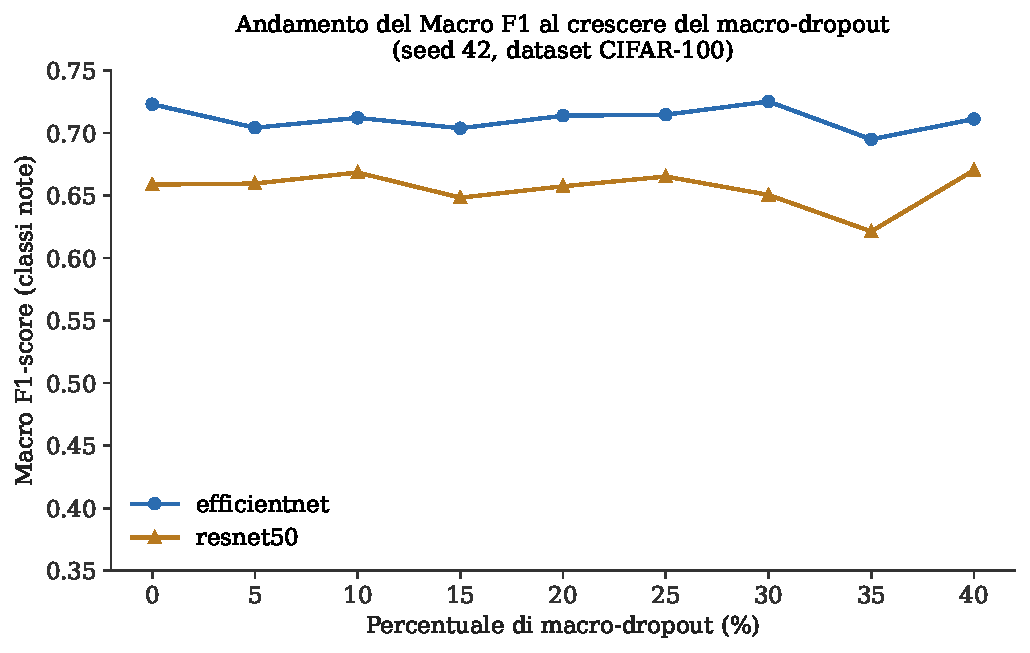
\includegraphics[width=0.75\textwidth]{figures/cifar_macro_dropout_f1.pdf}
    \caption{Andamento del Macro F1-score al variare della percentuale di macro-drop, per EfficientNet e ResNet50 sul dataset CIFAR-100 (seed 42).}
    \label{fig:macro-dropout-cifar}
\end{figure}

\begin{table}[!ht]
    \centering
    \small
    \caption{Accuracy, Precision e F1-score al variare della percentuale di macro-drop, per EfficientNet e ResNet50 sul dataset CIFAR-100 (seed 42).}
    \label{tab:metriche-cifar-macro}
    \begin{tabular}{llccc}
        \toprule
        \textbf{Modello} & \textbf{Drop \%} & \textbf{Accuracy} & \textbf{Precision} & \textbf{F1-score} \\
        \midrule
        \multirow{3}{*}{EfficientNet} & 0  & 0.723 & 0.738 & 0.723 \\
                                       & 20 & 0.714 & 0.728 & 0.714 \\
                                       & 40 & 0.712 & 0.725 & 0.711 \\
        \midrule
        \multirow{3}{*}{ResNet50}     & 0  & 0.659 & 0.689 & 0.659 \\
                                       & 20 & 0.655 & 0.680 & 0.657 \\
                                       & 40 & 0.672 & 0.694 & 0.670 \\
        \bottomrule
    \end{tabular}
\end{table}

I valori in Tabella~\ref{tab:metriche-cifar-macro} confermano il comportamento osservato graficamente, con variazioni minime tra lo $0\%$ e il $40\%$ di macro-drop per entrambe le architetture. 
Il risultato è coerente con quanto osservato sul dataset Oxford-IIIT Pet, ed è atteso per lo stesso motivo: la riduzione uniforme degli esempi per ciascuna classe non altera la difficoltà relativa del problema di classificazione.

\FloatBarrier

\subsection*{Analisi Micro-drop}
Come mostrato in Figura~\ref{fig:micro-dropout-cifar} e in Tabella~\ref{tab:metriche-cifar-micro}, anche su CIFAR-100 il micro-drop produce un trend di degradazione chiaro e monotono del Macro F1-score al crescere della percentuale di classi rimosse dal training, 
in linea con quanto osservato sul dataset Oxford-IIIT Pet.
\begin{figure}[htbp]
    \centering
    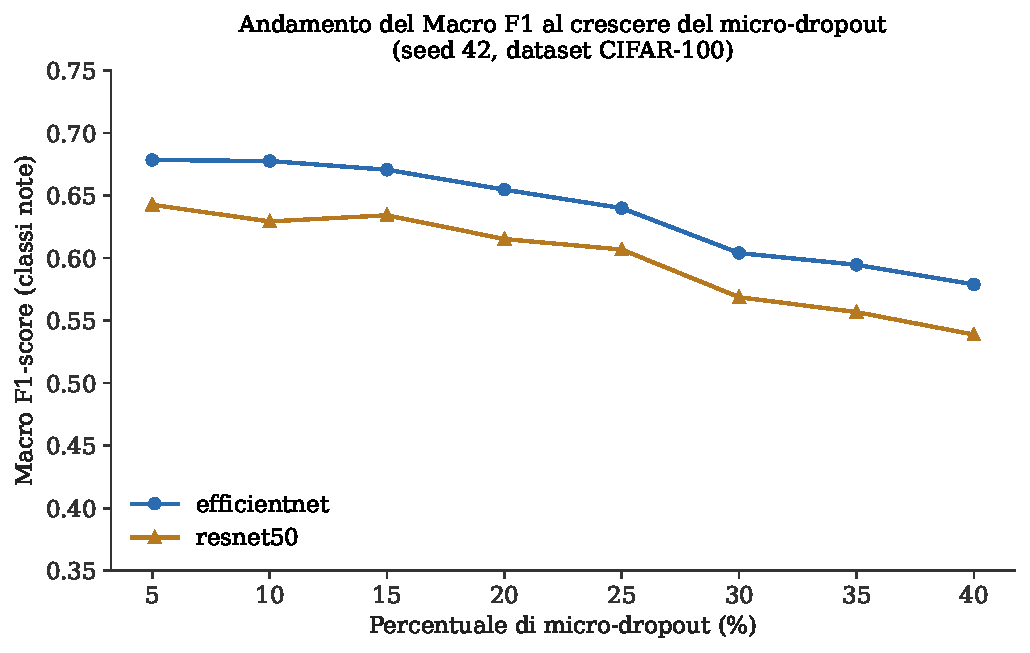
\includegraphics[width=0.85\textwidth]{figures/cifar_micro_dropout_f1.pdf}
    \caption{Andamento del Macro F1-score sulle classi note al variare della percentuale di micro-drop, per EfficientNet e ResNet50 sul dataset CIFAR-100 (seed 42).}
    \label{fig:micro-dropout-cifar}
\end{figure}
\begin{table}[!htb]
    \centering
    \small
    \caption{Accuracy (globale sull'intero test set), Precision (macro, classi note) e F1-score (macro, classi note) al variare della percentuale di micro-drop, per EfficientNet e ResNet50 sul dataset CIFAR-100 (seed 42).}
    \label{tab:metriche-cifar-micro}
    \begin{tabular}{llccc}
        \toprule
        \textbf{Modello} & \textbf{Drop \%} & \textbf{Accuracy} & \textbf{Precision} & \textbf{F1-score} \\
        \midrule
        \multirow{3}{*}{EfficientNet} & 0  & 0.723 & 0.738 & 0.723 \\
                                       & 20 & 0.579 & 0.620 & 0.655 \\
                                       & 40 & 0.452 & 0.489 & 0.579 \\
        \midrule
        \multirow{3}{*}{ResNet50}     & 0  & 0.659 & 0.689 & 0.659 \\
                                       & 20 & 0.542 & 0.595 & 0.615 \\
                                       & 40 & 0.412 & 0.469 & 0.539 \\
        \bottomrule
    \end{tabular}
\end{table}

Il confronto con i risultati ottenuti su Oxford-IIIT Pet (Sezione~\ref{sec:pet}) evidenzia un comportamento coerente tra i due dataset: in entrambi i casi il micro-drop causa una degradazione progressiva del Macro F1-score al crescere 
della percentuale di classi rimosse, sebbene con intensità diverse a seconda dell'architettura e del dataset considerati. 
Su CIFAR-100 il calo risulta particolarmente marcato oltre il $25\%$ di drop, con una perdita di circa $25$ punti percentuali di Accuracy (fino a $27.1$ per EfficientNet e $24.7$ per ResNet50) tra il caso baseline e il $40\%$ di rimozione. 
I due dataset vengono confrontati nella discussione (Sezione~\ref{sec:discussione}).

\FloatBarrier

\clearpage
\section{Discussione sui risultati ottenuti}
\label{sec:discussione}

Il confronto tra i due dataset conferma alcuni pattern comuni e ne evidenzia altri maggiormente specifici di ciascun dataset.

\textbf{Macro-drop.} Su entrambi i dataset la riduzione uniforme degli esempi per classe non produce un trend di degradazione riconoscibile: le oscillazioni osservate restano contenute (con un intervallo di variazione del Macro F1 compreso tra $0.028$ e $0.080$ per Pet e tra $0.030$ e $0.049$ per CIFAR-100), confermando che questo tipo di degradazione non altera sostanzialmente la difficoltà relativa del problema.

\textbf{Micro-drop.} Come mostrato in Figura~\ref{fig:confronto-pet-cifar}, la rimozione di intere classi produce una degradazione progressiva del Macro F1-score su entrambi i dataset, con un calo relativo compreso approssimativamente tra il $10\%$ e il $22\%$ dalla baseline al $40\%$ di drop, a seconda dell'architettura considerata. La differenza principale tra i due dataset risiede nel punto di partenza: CIFAR-100 presenta prestazioni di baseline significativamente inferiori a quelle di Pet ($\text{F1} \approx 0.68$ contro $\text{F1} \approx 0.85$), verosimilmente a causa della maggiore complessità del task ($100$ classi contro $37$ e risoluzione nativa delle immagini di soli $32\times32$ pixel che, pur interpolata a $224\times224$, offre un livello di dettaglio visivo intrinsecamente inferiore rispetto a Oxford-IIIT Pet). Questo comporta che, a parità di percentuale di drop, le prestazioni assolute su CIFAR-100 risultino inferiori a quelle registrate su Pet. Il confronto a parità di percentuale va comunque interpretato con cautela: su Oxford-IIIT Pet la percentuale di micro-drop è calcolata sulle sole immagini delle razze canine (Sezione~\ref{sec:degradazione}), per cui il $40\%$ corrisponde a circa il $27\%$ del training set e a $9$ razze su $37$, mentre su CIFAR-100 corrisponde a $40$ classi su $100$.

Si osserva inoltre che l'andamento della curva di degradazione è più irregolare su Pet, specialmente per ResNet50, mentre risulta più regolare e monotono su CIFAR-100. Questo potrebbe essere legato al numero maggiore di classi coinvolte in CIFAR-100, che rende l'effetto della rimozione di singole classi meno sensibile alla specifica combinazione di classi escluse a ciascuna soglia.

\begin{figure}[htbp]
    \centering
    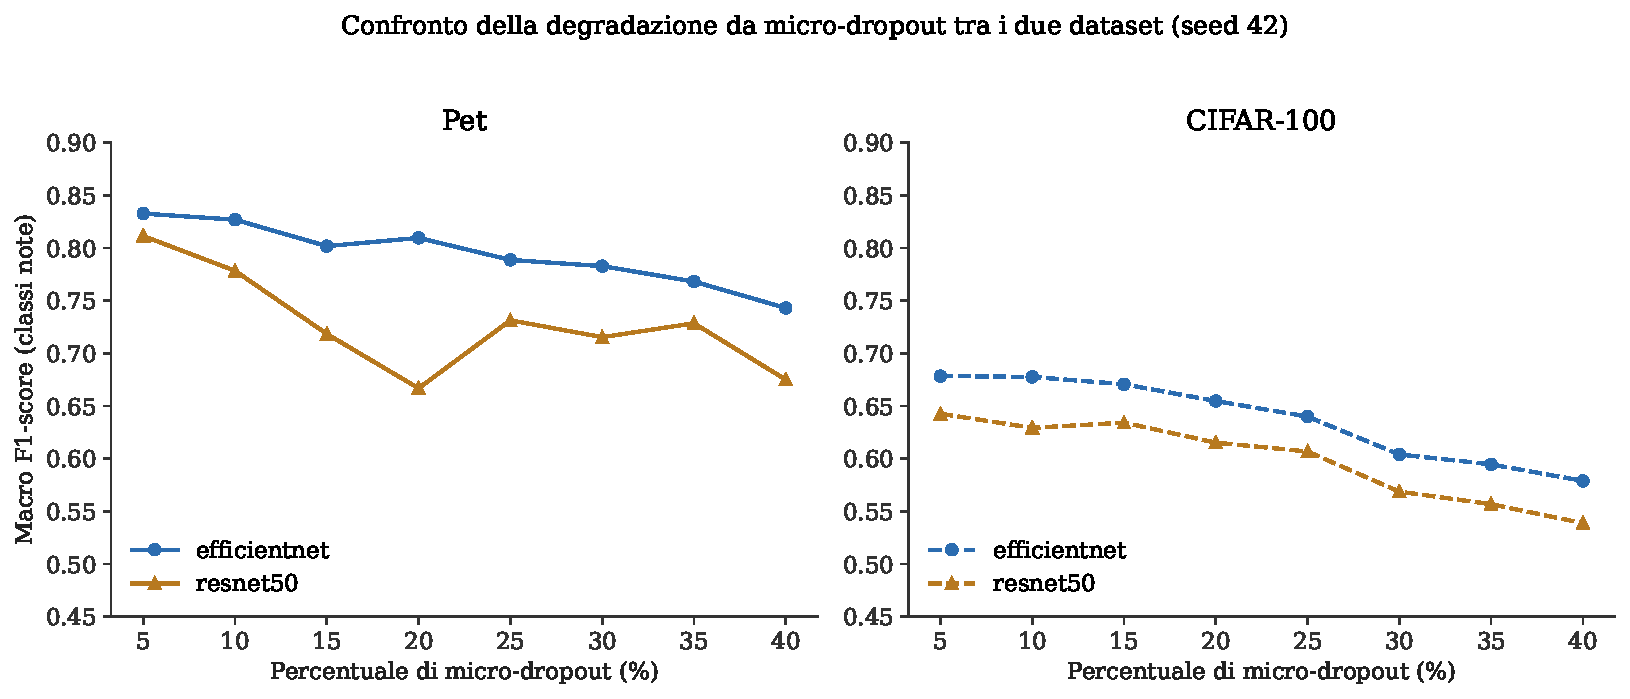
\includegraphics[width=\textwidth]{figures/confronto_pet_cifar_micro.pdf}
    \caption{Confronto diretto dell'andamento del Macro F1-score al crescere della percentuale di micro-drop tra i due dataset (seed 42).}
    \label{fig:confronto-pet-cifar}

\end{figure}

In entrambi i casi, il ranking tra le architetture si mantiene coerente: EfficientNet ottiene prestazioni superiori a ResNet50 a ogni livello di drop testato, su entrambi i dataset.
Si tratta tuttavia di un vantaggio in termini di prestazioni assolute, non di robustezza: in termini di calo relativo, su CIFAR-100 ResNet50 perde meno di EfficientNet ($-18.2\%$ contro $-19.9\%$), mentre su Pet il calo più contenuto è quello di DenseNet.